\chapter{Fundamentação Teórica e Metodologia}
\label{cap:fund_teorica}

\section{Métodos de Análise de Séries Temporais}
\label{sec:dmc}

O coeficiente \pdcca~\cite{Zebende2011} foi formulado tendo como bases o \emph{Detrended Fluctuation Analysis} (DFA)~\cite{Peng_1994} e o \emph{Detrended Cross-Correlation Analysis} (DCCA)~\cite{Podobnik2008}. O DFA é um método de análise de uma série temporal que fornece um parâmetro de auto-afinidade. O termo \emph{Detrended} refere-se a eliminação de uma tendência. O processo é executado em 6 passos:

\begin{enumerate}
    \label{list:dfa}
    \item Pegando a série temporal \(\{x_{i}\}\) com  \(i\) variando de  \(1\) à \(N\), a série integrada \(X_{k}\) é calculada por \(X_{k} = \sum_{i=1}^{k}\left[x_{i} - \langle x \rangle \right] \) com \(k\) também variando entre \(1\) e \(N\);
    \item A série  \(X_{k}\) é dividida em \(N - n\) caixas de tamanho \(n\) (escala temporal), cada caixa contendo \(n + 1\) observações, iniciando em \(i\) até \(i + n\);
    \item Para cada caixa um polinômio (geralmente de grau 1) é ajustado, gerando \(\widetilde{X}_{k, i}\) com \( i \le k \le (i + n) \) eliminando assim a tendência (detrended values);
    \item  para cada caixa é calculado: \(f_{DFA}^{2}(n, i) = \frac{1}{1+n} \sum_{k=i}^{i + n}(X_{k}-\widetilde{X}_{k, i})^{2}\)
    \item Para todas as caixas de uma escala temporal o DFA é calculado como: \(F_{DFA}(n) = \sqrt{\frac{1}{N - n} \sum_{i=1}^{N-n} f_{DFA}^{2}(n, i)}\);
    \item Para um número de diferentes escalas temporais (n), com valores possíveis entre \( 4 \le n \le \frac{N}{4}\), a função \(F_{DFA}\) é calculada para encontrar a relação entre \(F_{DFA} \times n\)
  \end{enumerate}

DFA também  representa as propriedades de auto-correlação de longo alcance de uma lei de potência~\cite{Zebende2013}. Se a correlação não existe, ou é uma correlação de curto alcance o valor do parâmetro \(\alpha = 0.5\), \(\alpha < 0.5\) indica antipersistência e \(\alpha > 0.5\) persistência.

O \(DCCA\) amplia o DFA para estabelecer a correlação entre duas séries temporais \cite{Podobnik2008}. O valor deste coeficiente tende a ser a média dos valores do DFA das duas séries e segue os 6 passos descritos abaixo:

\begin{enumerate}
  \label{list:dcca}
  \item Para duas séries temporais \(\{x_{i}\}\) e \(\{x_{i}\}\) com  \(i\) variando de  \(1\) à \(N\), as séries integradas \(X_{k}\) e \(Y_{k}\) são calculadas por \(X_{k} = \sum_{i=1}^{k}\left[x_{i} - \langle x \rangle \right] \) e \(Y_{k} = \sum_{i=1}^{k}\left[y_{i} - \langle x \rangle \right] \) com \(k\) também variando entre \(1\) e \(N\);
  \item As séries  \(X_{k}\) e \(X_{k}\) são divididas em \(N - n\) caixas de tamanho \(n\) (escala temporal), cada caixa contendo \(n + 1\) observações, iniciando em \(i\) até \(i + n\);
  \item Para cada caixa um polinômio (geralmente de grau 1) é ajustado, gerando \(\widetilde{X}_{k, i}\) para a primeira série e \(\widetilde{Y}_{k, i}\) para a segunda com \( i \le k \le (i + n) \) eliminando assim a tendência (detrended values);
  \item  Para cada caixa é calculado: $f_{DCCA}^{2}(n, i) = \frac{1}{1+n} \sum_{k=i}^{i + n}(X_{k}-\widetilde{X}_{k, i})(Y_{k}-\widetilde{Y}_{k, i})$
  \item Para todas as caixas de uma escala temporal a função $F_{DCCA}^{2}(n)$ é calculada por: $F_{DCCA}^{2}(n) = \frac{1}{N-n} \sum_{i=1}^{N-n} f_{DCCA}^{2}(n, i)$;
  \item Para um número de diferentes escalas temporais $(n)$, com valores possíveis entre \( 4 \le n \le \frac{N}{4}\), a função $F_{DCCA}^{2}(n)$ é calculada para encontrar a relação entre $F_{DCCA}^{2}(n) \times n$.
\end{enumerate}


Este coeficiente \(\lambda\) indica a existência de uma correlação entre duas séries regidas por leis de potência, mas não quantifica o nível desta correlação. O \emph{Detrended cross-correlation coefficient} ou \pdcca (equação \ref{eq_pdcca}) é um coeficiente que, variando entre -1 e 1, aponta ausência de correlação cruzada para valores próximos de zero, sendo maior a correlação quanto mais o valor se aproximar de 1 e maior a antecorrelação quanto mais o valor se aproximar de -1~\cite{Zebende2011}. 

\begin{equation}
\label{eq_pdcca}
\rho DCCA(n) = \frac{F_{DCCA}^2 (n)}{ F_{DFA1} (n) F_{DFA2} (n)}
\end{equation}

O método foi estatisticamente validado~\cite{PhysRevE.84.066118}, testado~\cite{vassolerZebende2012, Guedes2017, Ferreira2018},
e critérios para avaliação de relevância estatísticas do resultados foram desenvolvidos~\cite{Guedes2018,Guedes2018a}.

O \pdcca~foi estendido para calcular a correlação cruzada de múltiplas series temporais. Denominado \emph{Detrended Multiple Cross-Correlation Coefficient}~(\dmc), representa a generalização do \pdcca para múltiplas variáveis~\cite{Zebende2018}. Implementado com abordagem de janelas móveis~\cite{Guedes2021} e foi desenvolvido um teste estatístico para o coeficiente múltiplo~\cite{DaSilvaFilho2021}

O \dmc generaliza o \pdcca para tratar múltiplas séries temporais pela equação~\ref{eq:dmc}. Sendo $y$ uma serie temporal definida como variável dependente, $x_{i}$ um conjunto de $i$ séries temporais tomadas como variáveis independentes,  $\rho_{y,x_{i}}(n)$ o vetor contendo dos valores da função $F_{DCCA}^{2}(n)$ entre a serie $y$ e cada uma das séries $x_{i}$ e a matriz  $\rho^{-1}(n)$ definida pela equação~\ref{eq:dmc_mat_inv}

\begin{equation}\label{eq:dmc}
  {DMC}_{x}^{2}  \equiv \rho_{y,x_{i}}(n)^{T} \rho^{-1}(n) \rho_{y,x_{i}}(n)
\end{equation}


\begin{equation}\label{eq:dmc_mat_inv}
  \rho^{-1}(n) = \left(\begin{matrix} 
    1 & \rho_{x_{1},x_{2}}(n)                       &  \rho_{x_{1},x_{3}}(n) & \dots  &  \rho_{x_{1},x_{i}}(n) \\
    \rho_{x_{2},x_{1}}(n) & 1                       &  \rho_{x_{2},x_{3}}(n) & \dots  &  \rho_{x_{2},x_{i}}(n) \\
    \vdots                &  \vdots                 &  \vdots                & \dots  & \vdots \\
    \rho_{x_{i},x_{1}}(n) & \rho_{x_{i},x_{2}}(n)   &  \rho_{x_{i},x_{3}}(n) & \dots  &  1 \\
    \end{matrix}\right)^{-1}
\end{equation}

Já que muitos dos problemas que envolvem sistemas complexos lidam com mais de uma variável independente. E os sistemas e AM costumam abordar múltiplas variáveis independentes em suas buscas por padrões, dentre os métodos correlatos ao \pdcca, o \dmc apresenta as qualidades mais promissoras para embasar um algoritmo de AM.



\section{Aprendizado de Máquina e Redes Neurais Artificiais}
\label{sec:ml}

O aprendizado de máquina consiste na aplicação de algoritmos capazes de, através do processamento de um grande conjunto de dados, encontrar padrões, generalizar os critérios de encontrar padrões e prever eventos futuros\cite{bendavid2014}.

\begin{figure}[!htb]
	\centering
	\caption{Aprendizado de Máquina- diagrama conceitual}
	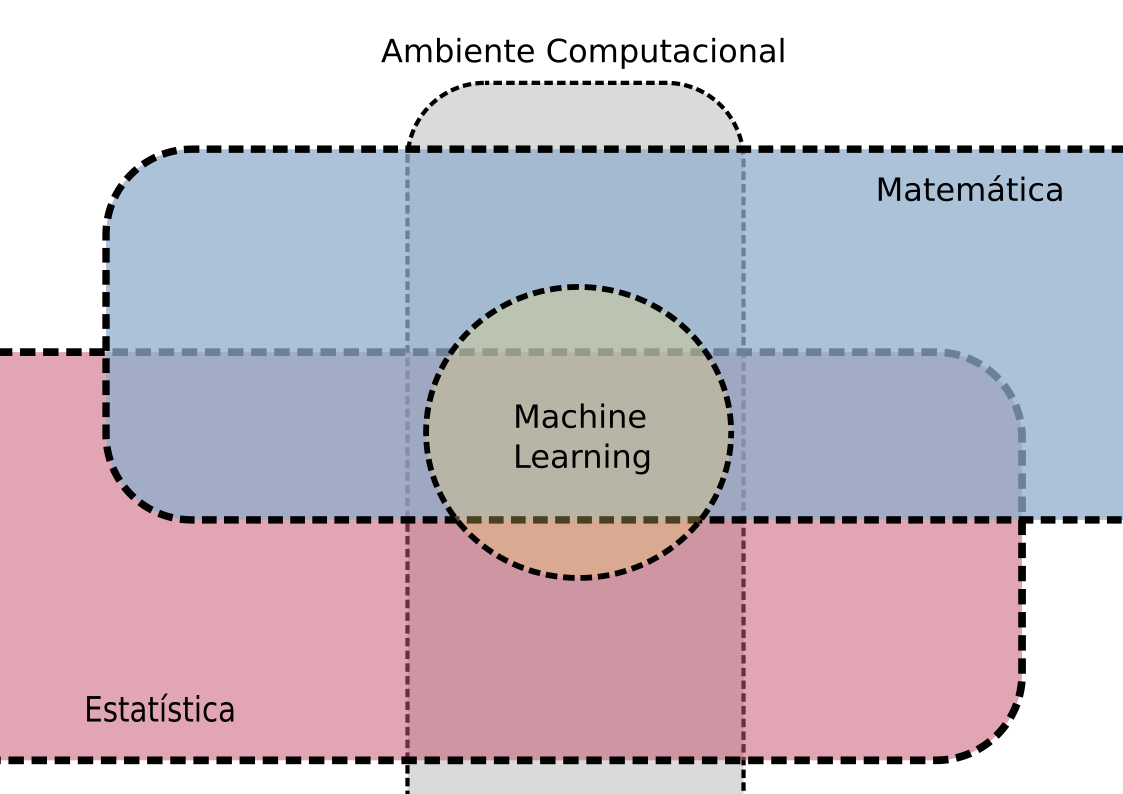
\includegraphics[width=.7\textwidth]{../Figures/ML/mat_est_ML.png}
	\\{\footnotesize Fonte: Elaborada Pelos Autores}
	\label{fig:MLdiag}
\end{figure}

Um campo guiado pela experimentação prática \cite{bishop2006}, pode ser definido pela busca em melhorar o desempenho computacional na realização de uma tarefa, através da experiência \cite{mitchell1997}. O desempenho nesta definição refere-se principalmente a quantificação dos acertos de acordo com uma métrica adequada à resolução do problema em questão e a experiência refere-se a um conjunto de dados coletados.

As tarefas em que os métodos de ML costumam superar os outros algoritmos também apresentam características peculiares: tratam de problemas fracamente definidos do ponto de vista matemático e/ou cujos métodos de resolução matemática são muito custosos do ponto de vista computacional em relação à velocidade necessária para a solução do problema na prática.

Reconhecimento facial e outras formas de interpretação de imagens, máquinas que andam, nadam e dirigem veículos, processamento de linguagem natural (falada e escrita) são exemplos de problemas fracamente definidos. Como definir com instruções de programação convencionais a sequência de instruções necessárias para ensinar um computador a resolver um dos destes problemas? Os algoritmos de ML tem apresentado boas respostas para este tipo de problema.

Redes neurais artificiais (RNA) representam um subgrupo dos métodos de ML inspirados no funcionamento das redes de neurônios estudadas pela Biologia, obtendo resultados robustos na aproximação de valores reais, discretos e  vetoriais~\cite{mitchell1997}.

Nesta analogia, para uma rede com apenas um neurônio, diversos atributos gravados em um conjunto de dados vão alimentar os dendritos do neurônio artificial. O núcleo do neurônio faria um somatório ponderado (o valor de cada atributo multiplicado por um valor de ponderação), além de um termo independente, conhecido como \emph{bias}. O valor final é submetido á uma função de ativação, que determina o valor que aproxima a função objetivo. O procedimento é análogo ao conceito de limiar de ativação, que transmite um impulso nervoso pelo axônio de um neurônio real. 

O treinamento de uma RNA consiste em receber parte das observações do conjunto de dados é otimizar o valor dos pesos para obter o melhor valor da métrica de validação possível. Após o treinamento, um subgrupo das observações que não foi usada no treinamento, é utilizado para  a etapa de testes (ou validação) onde é medido o grau de acerto dos valores aproximados em relação aos valores medidos e a capacidade de generalização da rede, ou seja, a capacidade do modelo de lidar com dados novos.

Os atributos podem ser valores de entrada para diversos neurônios em paralelo, formando uma camada. As camadas podem ser entradas de outras camadas antes do valor final (camada de saída) da aproximação. Quando existem camadas entre a de entrada e a de saída, se utiliza a terminologia \emph{deep learning}. 

Para simulações de dados sequenciais, como as séries temporais, arquiteturas especificas de RNA foram desenvolvidas. As \emph{Recurent Neural Networks}, propostas por \citeonline{Rumelhart1986we}, as RNN aplicam o conceito de \emph{backpropagation} para lidar com dados sequenciais e séries temporais. Divergindo das arquiteturas de \emph{feedforward}, onde as saídas de uma camada servem como entradas de camadas seguintes (imediatas ou não), as redes que apicam \emph{backpropagation} usam saídas de determinados neurônio seja utilizada como entrada dele mesmo, de outro neurônio da mesma camada ou de uma camada anterior. Isso permite que, em uma série temporal onde se pretende prever mais de uma unidade de tempo a frente, uma unidade prevista possa ser utilizada pra prever o valor da unidade seguinte
 
Muitas variantes das RNN foram propostas para aproximar resultados e fazer previsões em séries temporais e dados sequenciais, dentre os mais utilizados estão as LSTM \cite{Hochreiter1997}, que procura avaliar, durante o treinamento da rede, qual o número ideal de medições anteriores à ser usado para prever os valores de um determinado número de passos seguintes. Para tanto, utiliza-se de portões (\emph{gates}) que controlam se determinado valor passado será ou não utilizado na definição dos pesos. Mais recentemente surgiram as GRU \cite{Cho2014} como um subconjunto das LSTM, implementados com bastante sucesso em diversos problemas práticos.

Apesar de muitas das fases de implementação de uma RNA serem guiadas por experimentação prática, do ponto de vista matemático, esses modelos são representados por equações diferenciais, cujo entendimento pode produzir \emph{insights} no tratamento dos dados e definição da arquitetura \cite{Sherstinsky2020}.
